\documentclass[conference]{IEEEtran}
\ifCLASSINFOpdf

\newcommand{\redcolor}[1]{\textcolor{red}{#1}}

\newcommand{\figref}[1]{Figure~\ref{#1}}
\newcommand{\secref}[1]{Section~\ref{#1}}
\newcommand{\tabref}[1]{Table~\ref{#1}}
\newcommand{\algoref}[1]{Algorithm~\ref{#1}}

\usepackage{subfig}
\usepackage{caption}
\usepackage{url}
\usepackage{epstopdf}
\usepackage{graphicx}
%\usepackage[pdftex]{graphicx}
% % declare the path(s) where your graphic files are
%\graphicspath{{../figures/}}
%  % and their extensions so you won't have to specify these with
%  % every instance of \includegraphics
%\DeclareGraphicsExtensions{.pdf,.jpeg,.png}
\else
\fi
% *** MATH PACKAGES ***
%
%\usepackage[cmex10]{amsmath}
% *** SPECIALIZED LIST PACKAGES ***
%
%\usepackage{algorithmic}

% *** ALIGNMENT PACKAGES ***
%
%\usepackage{array}
%\usepackage{mdwmath}
%\usepackage{mdwtab}
%\usepackage{eqparbox}
% *** SUBFIGURE PACKAGES ***
%\usepackage[tight,footnotesize]{subfigure}
%\usepackage[caption=false]{caption}
%\usepackage[font=footnotesize]{subfig}

% *** FLOAT PACKAGES ***
%
%\usepackage{fixltx2e}
%\usepackage{stfloats}
% *** PDF, URL AND HYPERLINK PACKAGES ***
%\usepackage{url}
% correct bad hyphenation here
\hyphenation{op-tical net-works semi-conduc-tor}


\begin{document}
%
% paper title
% can use linebreaks \\ within to get better formatting as desired
\title{Back to Basics: Simplifying Non-Intrusive Appliance Load Monitoring Using Combinatorial Optimization}


% author names and affiliations
% use a multiple column layout for up to three different
% affiliations
\author{\IEEEauthorblockN{Author1}
\IEEEauthorblockA{Indraprastha Institute of Information Technology\\
India\\
}
\and
\IEEEauthorblockN{Author2}
\IEEEauthorblockA{Twentieth Century Fox\\
Springfield, USA\\
Email: homer@thesimpsons.com}
\and
\IEEEauthorblockN{James Kirk\\ and Montgomery Scott}
\IEEEauthorblockA{Starfleet Academy\\
San Francisco, California 96678-2391\\
Telephone: (800) 555--1212\\
Fax: (888) 555--1212}}
% make the title area
\maketitle


\begin{abstract}
%\boldmath
Non-Intrusive appliance load monitoring (NIALM) is the process of disaggregating the overall electricity usage into constituent appliances. In this paper we extend the Combinatorial Optimization (CO) approach for disaggregation, which was originally proposed in the seminal work on NIALM, in following two ways: 1) Breaking the problem into subproblems and reducing the state space; 2) Applying additional constraints backed by sound domain expertise. We evaluate our approach using REDD dataset and show practical problems which need to be solved while dealing with the dataset. We also propose a metric for evaluating NILM, which we believe overcomes many shortcomings of commonly used metrics.
\end{abstract}
\IEEEpeerreviewmaketitle



\section{Introduction}
% no \IEEEPARstart
\begin{itemize}
\item Motivate the importance of energy consumption in building
\item Motivate that appliance level information is crucial - detailed feedback and optimized decision making \cite{darby}
\item Challenges with getting appliance level information - introduce NIALM~\cite{hart}
\item introduce your proposed approach
\item Enumerate the contributions
\end{itemize}

Primary contributions of our work are:
\begin{itemize}
\item Fill it up with 2-3 crisp points
\end{itemize}
Open source implementation of the proposed work is released for comparative analysis with other NIALM approaches as an IPython notebook\footnote{\url{http://www.ipython.org}}. We believe this is the first extensive release of a generic NIALM

\section{Related work}
NIALM has been well studied in the recent past and survey papers \cite{survey1,survey2,survey3} present its classification across various dimensions. Following are three important classification dimensions:
\begin{itemize}
\item \textbf{Frequency of data collection}: Approaches such as harmonic analysis require data to be sampled at more than a thousand samples a second. Whereas approaches 
\item \textbf{Supervised/Unsupervised}: 
\end{itemize}
When you do the comparison, bring up how is your work different rather than just saying X did A and Y did B.
\begin{itemize}
\item Classification of different NIALM approaches - High/Low frequency, Time/Frequency domain analysis, supervised/unsupervised~\cite{survey1,survey2,survey3}.

For a more detailed overview the reader is referred to the above mentioned survey papers.

\item Discuss the modeling approaches that are used
\begin{itemize}
\item Additive Factorial HMM
\item Difference HMM \cite{parson2012_aaai}
\end{itemize}

\item Datasets used: Recent datasets have spurred this field
\begin{itemize}
\item REDD \cite{redd}
\item Blued \cite{blued_cmu}
\item Smart* \cite{smart}
\end{itemize}

\end{itemize}



% An example of a floating figure using the graphicx package.
% Note that \label must occur AFTER (or within) \caption.
% For figures, \caption should occur after the \includegraphics.
% Note that IEEEtran v1.7 and later has special internal code that
% is designed to preserve the operation of \label within \caption
% even when the captionsoff option is in effect. However, because
% of issues like this, it may be the safest practice to put all your
% \label just after \caption rather than within \caption{}.
%
% Reminder: the "draftcls" or "draftclsnofoot", not "draft", class
% option should be used if it is desired that the figures are to be
% displayed while in draft mode.
%
%\begin{figure}[!t]
%\centering
%\includegraphics[width=2.5in]{myfigure}
% where an .eps filename suffix will be assumed under latex, 
% and a .pdf suffix will be assumed for pdflatex; or what has been declared
% via \DeclareGraphicsExtensions.
%\caption{Simulation Results}
%\label{fig_sim}
%\end{figure}

% Note that IEEE typically puts floats only at the top, even when this
% results in a large percentage of a column being occupied by floats.


% An example of a double column floating figure using two subfigures.
% (The subfig.sty package must be loaded for this to work.)
% The subfigure \label commands are set within each subfloat command, the
% \label for the overall figure must come after \caption.
% \hfil must be used as a separator to get equal spacing.
% The subfigure.sty package works much the same way, except \subfigure is
% used instead of \subfloat.
%
%\begin{figure*}[!t]
%\centerline{\subfloat[Case I]\includegraphics[width=2.5in]{subfigcase1}%
%\label{fig_first_case}}
%\hfil
%\subfloat[Case II]{\includegraphics[width=2.5in]{subfigcase2}%
%\label{fig_second_case}}}
%\caption{Simulation results}
%\label{fig_sim}
%\end{figure*}
%
% Note that often IEEE papers with subfigures do not employ subfigure
% captions (using the optional argument to \subfloat), but instead will
% reference/describe all of them (a), (b), etc., within the main caption.


% An example of a floating table. Note that, for IEEE style tables, the 
% \caption command should come BEFORE the table. Table text will default to
% \footnotesize as IEEE normally uses this smaller font for tables.
% The \label must come after \caption as always.
%
%\begin{table}[!t]
%% increase table row spacing, adjust to taste
%\renewcommand{\arraystretch}{1.3}
% if using array.sty, it might be a good idea to tweak the value of
% \extrarowheight as needed to properly center the text within the cells
%\caption{An Example of a Table}
%\label{table_example}
%\centering
%% Some packages, such as MDW tools, offer better commands for making tables
%% than the plain LaTeX2e tabular which is used here.
%\begin{tabular}{|c||c|}
%\hline
%One & Two\\
%\hline
%Three & Four\\
%\hline
%\end{tabular}
%\end{table}

\section{NIALM}
Discuss in brief the NIALM problem
\subsection{Terminologies/ Notations}
Borrow the notation used by Parson and Hart.
\begin{itemize}
\item Input: Aggregate power sequence: $x=\{ x_1,..,x_T\}$
\item Infer: Power draw by constituent appliance: $y_n=\{y_{1,n},..y_{T,n}\}$
\item Time slice: $t\in {1,..T}$
\item Appliance: $n\in{1,..N}$
\item Appliance state: $z_n=\{z_1,..z_T\}$
\end{itemize}

\subsection{NIALM using combinatorial optimization}
This approach resembles subset sum problem and tries to minimize the difference of total observed power from the sum of various possible subsets coming from various combinations of appliances in different states. For each appliance we assume \textbf{K} states and at a given time, an appliance can only be in a single state. This is given as: 
$z_{t,n,k}\in\{0,1\} $ and, $$\sum\limits_{k=1}^{k=K} z_{t,n,k}=1$$The power drawn by each appliance is given by:
$$\mu_n=\{\mu_{n,1},..\mu_{n.K}\}$$ Thus, CO can be formulated as:
$$z_t=arg min_{z_t}|x_t-\sum\limits_{n=1}^{N}\sum\limits_{k=1}^{K}z_{t,n,k}\mu_{n,k}|$$

\begin{itemize}
\item Statespace is $K^N$
\item We assign different loads to different mains, $N_i$ loads to $Mains_i$, $\sum\limits_{1}^{p}{N_i}=N$. Now different state spaces are
$K^{N_1}$.... We can define the overall state space as $\max{K^{N_i}}$

As a practical example, two mains, 20 appliance, state space before = $2^{20}$. After = $2^{10}$. Exponential reduction in state space.
\end{itemize}

Highlight what is the simplification you are bringing forth.

\section{Name of algorithm as section label}
Think of appropriate name for your approach
\textbf{Flowchart- TO go as image/flow diagram}
\begin{enumerate}
\item Data Preprocessing
\begin{enumerate}
\item Aligning Mains and Appliance Level data
\item Down sampling to 1 minute resolution
\end{enumerate}
\item Load Assignment based on 
\begin{enumerate}

\item Appliance usage times
\item Appliance Periodicity
\item Appliance Power threshold
\item Correlation amongst different appliance usage

\end{enumerate}
\item Data Recalibration using the following
\begin{enumerate}
\item Step changes occurring in Mains vs Appliances
\item Isolating single appliance usage
\end{enumerate}
\item Appliance states identification using clustering (Possibly talk about unbalanced data, but leave it for future work)
\item State space creation
\item Applying CO for different mains
\item Find energy distribution by appliance and assign weights (To be used in results)

\end{enumerate}


Explanation of above steps
\subsection{Data Pre processing}
\begin{itemize}
\item Aligned data
\item Down sampling and why it is needed
\begin{itemize}
\item Sub metered data collected sometimes at 3s sometimes at 4 s
\item Getting rid of transients, also suggested by Hart
\item Reducing power fluctuations occurring due to voltage fluctuations. Put figure showing reduction in transients and signal smoothing
\end{itemize}
\end{itemize}
\begin{figure} 
	
    \subfloat[\scriptsize Filtering startup transients]{
    \includegraphics[scale=0.1]{./figures/downsampled_1.png}}
    \subfloat[\scriptsize Filtering voltage fluctuations and oscillations]{
        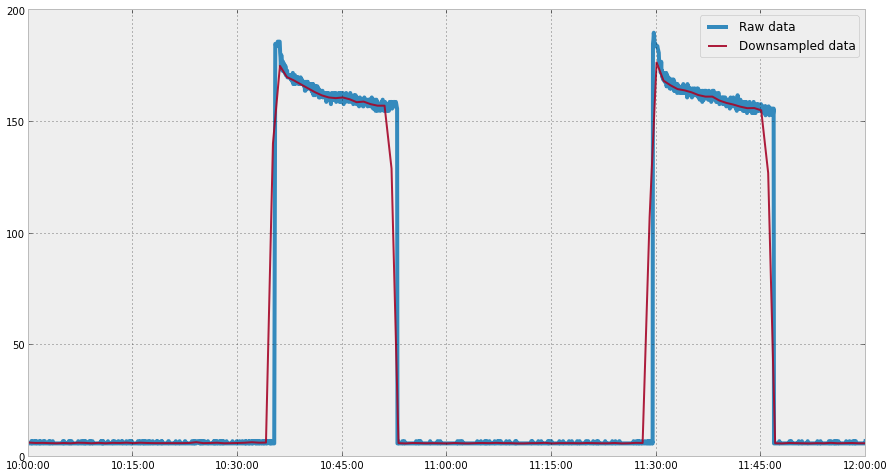
\includegraphics[scale=0.1]{./figures/downsampled_2.png}}
  	\caption{Effect of downsampling appliance data}
    \label{fig:downsampling}
\end{figure}

%\begin{figure*}[!t]
%\centerline{\subfloat[Case I]\includegraphics[width=2.5in]{downsampled_1}%
%\label{fig_first_case}}
%\hfil
%\subfloat[Case II]{\includegraphics[width=2.5in]{subfigcase2}%
%\label{fig_second_case}}}
%\caption{Simulation results}
%\label{fig_sim}
%\end{figure*}

\subsection{Load assignment}
Draws inspiration from work by Parson et. al \cite{parson2012_aaai}. From prior knowledge we divide the loads into two different categories: Periodic such as refrigerator and non periodic such as Television.

\section{Evaluation}
\subsection{About Dataset}

We use REDD dataset \cite{redd} for validating our algorithms. This dataset contains power and voltage data for mains (2 phases) as well as appliances from 6 homes in Boston area collected in the summer of 2011. The data is made available as raw, high frequency (sampled at 15 KHz) and low frequency (Mains at 1 Hz, appliances at ~.3 Hz). Considering the practical implications of residential smart meter installation, we believe that low frequency data represents the most realistic scenario and thus we use this data for analysis. \figref{fig:breakdown} shows 6 hourly breakdown of energy consumption across the different mains in Home 2 .


\begin{figure} 
	
    \subfloat[\scriptsize Mains 1]{
    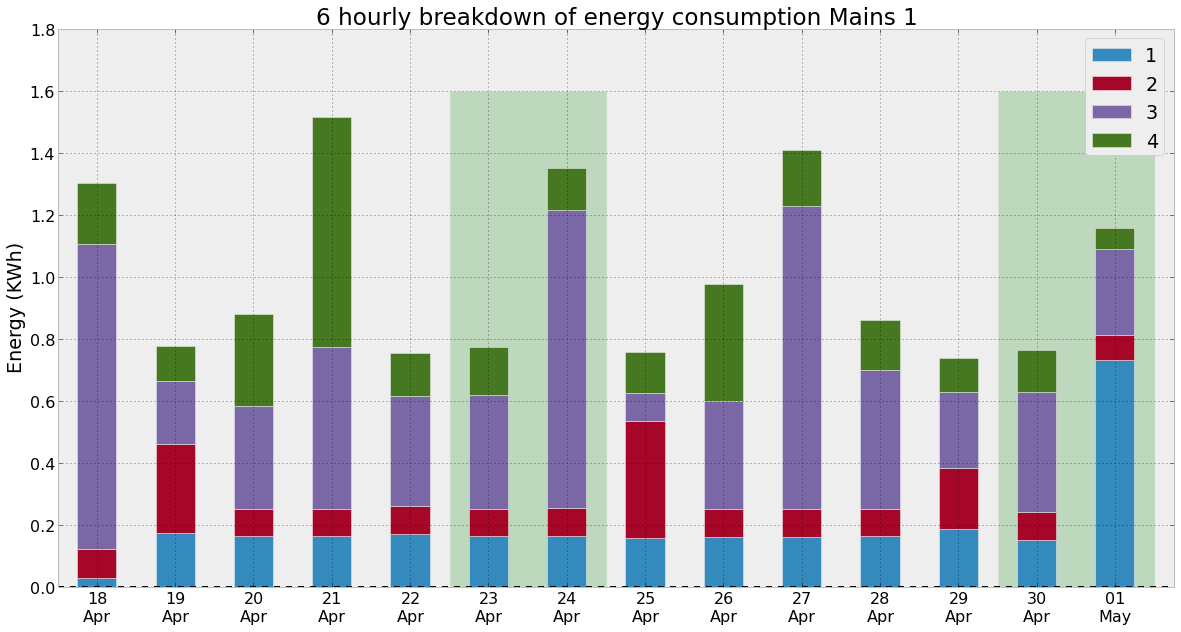
\includegraphics[scale=0.1]{./figures/mains_1_6hr.png}}
    \subfloat[\scriptsize Mains 2]{
        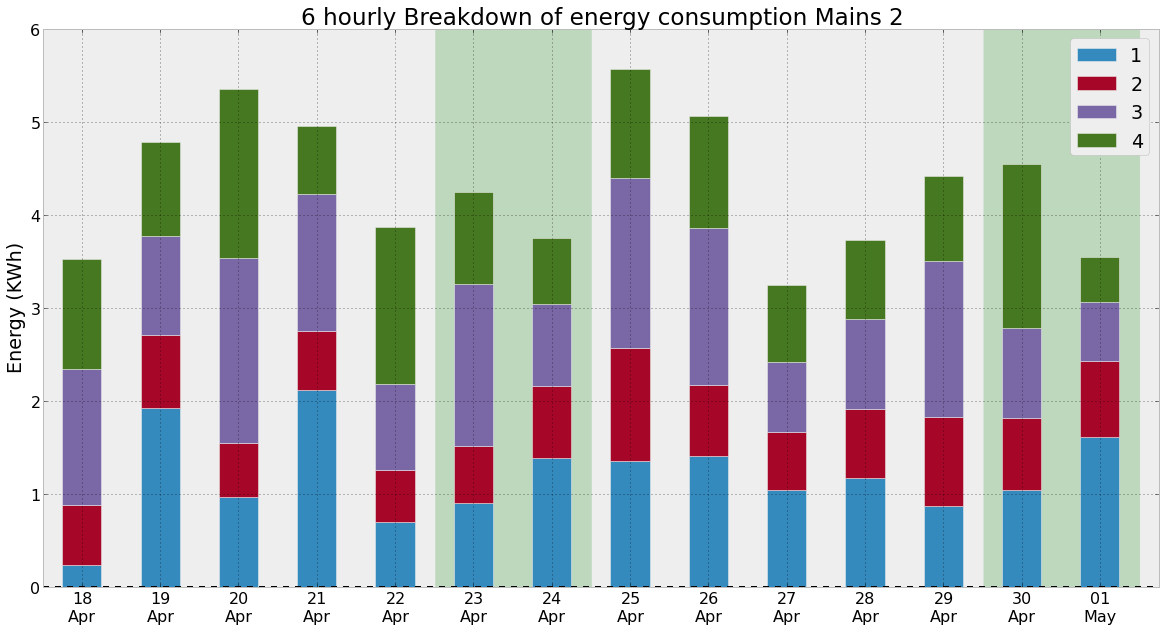
\includegraphics[scale=0.1]{./figures/mains_2_6hr.png}}
  	\caption{6 hourly energy usage breakdown Home 2}
    \label{fig:breakdown}
\end{figure}

\subsection{Evaluation Metric}

Commonly used metrics such as accuracy, sensitivity and specificity can be misleading when applied to NILALM. \figref{fig:confusion} jkj
%\begin{figure}
%\centering 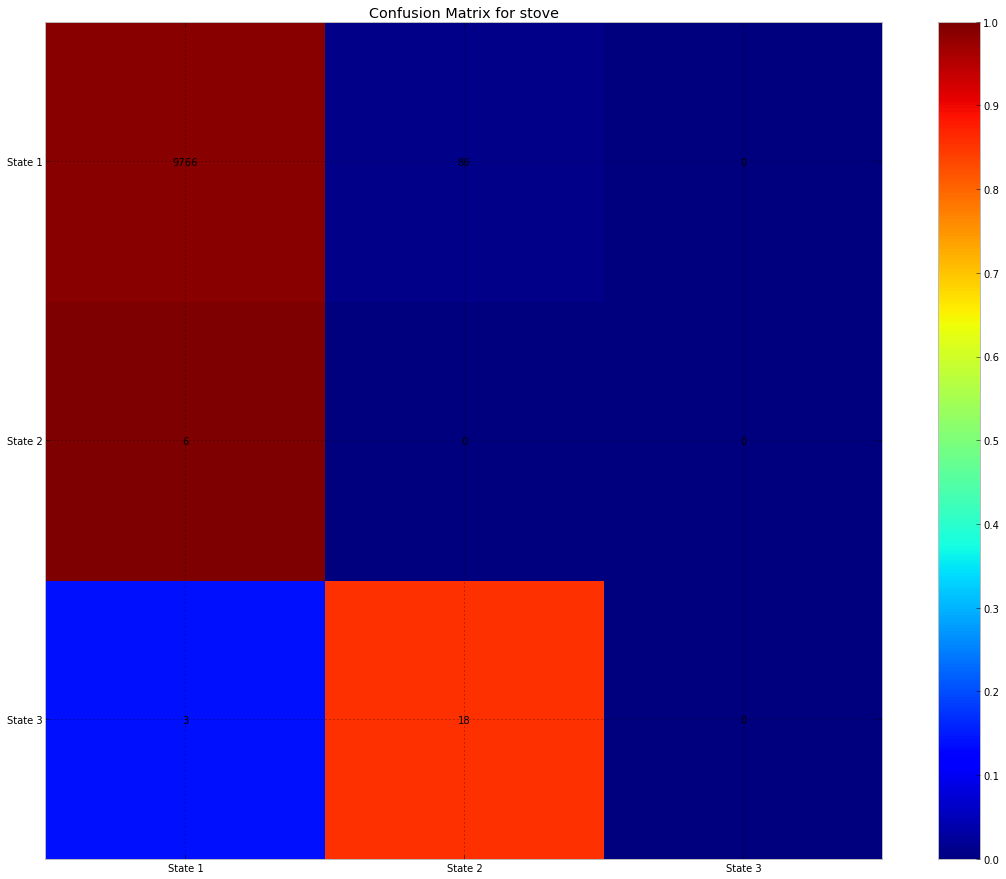
\includegraphics[scale=0.1]{./figures/confusion_stove.png}
%  	\caption{Confusion Matrix showing predicted state accuracy for Stove}
%    \label{fig:confusion}
%\end{figure}
    \begin{itemize}
\item Image of confusion matrix
\item Show confusion matrix and argue that accuracy can be misleading, state 0 dominates in all appliances and will most probably always be predicted correctly
\item Hart pointed towards residual power as an evaluation metric, REDD paper talks about \% of energy recovered
\item METRIC 1: Given an appliance having $m$ states, we propose power weighted appliance accuracy, as follows
$Appliance Accuracy = \frac{\sum\limits_{i=1}^{m} Accuracy(i)*Power(i)}{Power(i)} $
\item METRIC 2: In this we also take into consideration the amount of time an appliance is in a particular state
\item Overall Accuracy : Based on energy weights of different appliance, for instance .4* Fridge +.2*Light+...
This is important since it shows the relative importance of larger loads 
\item Switch continuity
\end{itemize}

\subsection{Empirical Analysis}
We analyze data from Home 2 of the REDD dataset and believe that the same analysis can be easily repeated across multiple homes. We do this to compare our results against the Factorial Hidden Markov approach used by Kolter et al. \cite{redd} on the same home.

\begin{itemize}
\item Table on Cluster assignment
\item Table on Results
\item Table on on /off periods
\item Table on switch continuity
\end{itemize}



\section{Conclusion}
The conclusion goes here.
We also provide mains load assignment of all 6 homes from REDD to further the research in this direction.

\section{Future Work}
\begin{itemize}

\item Applying model on noisy datasets
\item 2 D CO (when Real and Reactive Power are known)
\item Factoring in Time of Day etc.
\item Factoring in Appliance Correlation
\item Factor in switch continuity, essentially leads to Factorial HMM
\item Distributed NILM
\item Adaptive Learning
\end{itemize}

\section*{Acknowledgment}
The authors would like to thank TCS Research and Development for supporting the first author through PhD. fellowship. We would also like to thank NSF- DEITy for funding the project.
\bibliographystyle{IEEEtran}
\bibliography{IEEEabrv,references}

\end{document}


